\section{Definición de grafo}
\label{sec:definicion_de_grafo}

Un grafo es un objeto matemático en el cual arcos conectan pares de vértices. Formalmente:

\begin{definicion}{Grafo}{grafo}
  Un \concept{grafo} $G$ es un par ordenado de conjuntos disjuntos $(V, E)$ tal que $V$ es un conjunto de \concept{vértices} o \concept{nodos} y $E$ es un conjunto de \concept{aristas} o \concept{arcos} que conectan pares de vértices.
\end{definicion}

Gráficamente, los vértices se representan por puntos y los arcos se representan por segmentos de recta que los conectan. El siguiente es un ejemplo de grafo cada vértice están marcado con una letra:

\begin{center}
  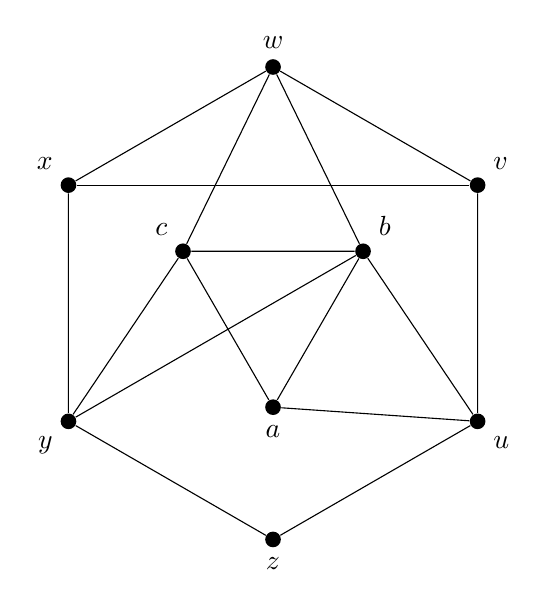
\begin{tikzpicture}[scale=1.2,
    vertex/.style={circle, fill=black, inner sep=2pt}]
    % Outer vertices (on c circle of radius 2.5)
    \node[vertex, label=above:$w$]      (w) at (90:2.5)  {};
    \node[vertex, label=above right:$v$](v) at (30:2.5)  {};
    \node[vertex, label=below right:$u$](u) at (330:2.5) {};
    \node[vertex, label=below:$z$]      (z) at (270:2.5) {};
    \node[vertex, label=below left:$y$] (y) at (210:2.5) {};
    \node[vertex, label=above left:$x$] (x) at (150:2.5) {};
    % Inner vertices (on c circle of radius 1.1)
    \node[vertex, label=above left:$c$] (c) at (150:1.1) {};
    \node[vertex, label=below:$a$]      (a) at (270:1.1) {};
    \node[vertex, label=above right:$b$](b) at (30:1.1)  {};
    % Outer cycle
    \draw (y)--(z)--(u)--(v)--(w)--(x)--(y);
    % Outer diagonal
    \draw (x)--(v);
    % Inner triangle
    \draw (c)--(b)--(a)--(c);
    % Outer-to-inner spokes
    \draw (w)--(c) (w)--(b);
    \draw (y)--(c) (y)--(b);
    \draw (u)--(b) (u)--(b);
    \draw (a)--(u);
  \end{tikzpicture}
\end{center}

En ocasiones es útil enfatizar que $V$ es el conjunto de vértices de $G$ escribiendo $V(G)$, para no confundirlo con un posible conjunto de vértices $V(H)$ del grafo $H$. Lo mismo se puede hacer para $E(G)$ y $E(H)$.

Salvo que explícitamente se diga lo contrario, en estos apuntes se estudian \concept{grafos finitos}, en los que los conjuntos $V$ y $E$ son finitos.

\subsection{Tipos de grafo}
\label{sec:tipos_de_grafo}

\subsubsection{Dirigido o no dirigido}
\label{sec:dirigido_vs_no_dirigido}

Dependiendo de la estructura del conjunto de arcos, un grafo es dirigido o no dirigido:

Si los arcos de un grafo se dirigen de un vértice hacia otro, el grafo es \concept{dirigido}. En ese caso, $E \subseteq V \times V$ y los arcos son pares \emph{ordenados} de la forma $(u,v)$.

Si los arcos de un grafo no tienen dirección, el grafo es \concept{no dirigido}. Si $\binom{V}{2}$ denota el conjunto de subconjuntos de cardinalidad $2$ de $V$, entonces $E \subseteq \binom{V}{2}$, es decir, los arcos son pares \emph{no ordenados} de la forma $\{u,v\}$.

\subsubsection{Simple o multigrafo}
\label{sec:simple_o_multigrafo}

Un \concept{lazo} (\textit{loop}) es un arco que conecta un vértice consigo mismo, de la forma $\{v, v\}$ en un grafo no dirigido o $(v, v)$ en un grafo dirigido.

Un grafo es \concept{simple} si no tiene lazos y además hay a lo sumo un arco entre cada par de vértices. Salvo que explícitamente se diga lo contrario, los conceptos en estos apuntes suponen grafos simples.

Si un grafo puede tener lazos, se dice que es un \concept{grafo simple con lazos}. Su conjunto de arcos es de la forma $E \subseteq \begin{pmatrix} V\\2 \end{pmatrix} \cup \{\{a\}|a\in V\}$ y los lazos son conjuntos \textit{singleton} con un solo vértice.

Si un grafo puede tener múltiples arcos entre el mismo par de vértices, se dice que es un \concept{multigrafo}. En ese caso, $E \subseteq \begin{pmatrix} V\\2 \end{pmatrix} \times \mathbb{N}$ es el conjunto de arcos, de la forma $(\{u, v\}, n)$ donde $u,v\in V$ y $n \in \mathbb{N}$. El número asociado a cada arco no es un peso, a diferencia de en un \hyperref[sec:grafos_ponderados]{grafo ponderado}. Es un diferenciador, para discernir entre arcos que conectan el mismo par de vértices.

\subsubsection{Grafos ponderados}
\label{sec:grafos_ponderados}

Un grafo \concept{ponderado} es una tripla $G = (V, E, w)$, donde $(V, E)$ es un grafo (de cualquiera de los tipos anteriormente definidos) y $w\colon E \to \mathbb{R}$ es una función de pesos que asigna un número real a cada arco.
